%% See http://www.oxfordjournals.org/our_journals/bioinformatics/for_authors/general.html for author information

\documentclass{bioinfo}

\def\TTra{\textsuperscript{\tiny{\texttrademark}\,}}

\copyrightyear{2011}
\pubyear{2011}

\hyphenation{
be-tween
trans-late
i-den-ti-fiers
el-e-ments
path-way
con-tent
re-search-ers
in-di-vid-u-al
de-scrip-tion
}

\begin{document}
\application
\firstpage{1}

\title[KEGGtranslator]{KEGGtranslator: visualizing and translating the KEGG PATHWAY database} %% TODO: Irgendwas mit modelling oder simulation oder so klingt besser.
\author[Wrzodek \textit{et~al}]{Clemens Wrzodek\,$^{1,}$\footnote{to whom correspondence should be addressed}, Andreas Dr\"ager\,$^{1,*}$ and Andreas Zell\,$^1$}
\address{$^{1}$Center for Bioinformatics Tuebingen (ZBIT), University of Tuebingen, Sand 1, 72076 T\"ubingen, Germany}

\history{Received on XXXXX; revised on XXXXX; accepted on XXXXX}

\editor{Associate Editor: XXXXXXX}

\maketitle

\begin{abstract}

\section{Summary:}
Nowadays, the KEGG PATHWAY database provides a widely used service for pathway-based information. It contains manually drawn pathway maps with information about the genes, reactions and relations contained therein. To store these pathways, KEGG uses an own XML-format. Parsers and translators are needed to process the pathway maps for usage in other applications and algorithms.


We have developed KEGGtranslator, which is an easy-to-use stand-alone application that can visualize and convert KGML formatted XML-files into multiple output formats. Unlike other translators, KEGGtranslator supports a plethora of output formats, is able to augment the information in translated documents (e.g., MIRIAM annotations) beyond the scope of the KGML document, and amends missing components to fragmentary reactions within the pathway to allow simulations on those.

% [is able to complete [...] beyond the scope of the XML-document] by retrieving additional pathway information from the internet.

%Es gibt ein paar andere translator, aber...
%XML-grafisch ok, f�r simmulationen nicht so toll.
%Translator nutzt KegggAdaptor, kann RkT vervollst�ndigung, ist Stand-Alone-Application

\section{Availability:}
KEGGtranslator is freely available as a webstart application and for download at \href{http://www.cogsys.cs.uni-tuebingen.de/software/KEGGtranslator/}{http://www.cogsys.cs.uni-tuebingen.de/software/KEGGtranslator/}. KGML files can be downloaded within the application or manually from \href{ftp://ftp.genome.jp/pub/kegg/xml/kgml}{ftp://ftp.genome.jp/ pub/kegg/xml/kgml}.


\section{Contact:} \href{clemens.wrzodek@uni-tuebingen.de}{clemens.wrzodek@uni-tuebingen.de}
\end{abstract}

%% TODO: Availability and Implementation section (Java, runs on most OS, blablabla)

\section{Introduction}

%Aufbau:
%Kern problem: KGML-Format der Pathways.
%1. Kegg ist toll weil...
%2. Man k�nnte so viel tun (Bilder, Simulation, Graph-Anwendungen(Operation), St�chiometrische analysen (zB lineare abh�ngigkeiten), GSEA)
%3. Aber das Format ist ungeeignet
%4. Daher gibt es mehrere Konverter, die folgendes k�nnen
%5. Das gen�gt nicht weil
%6. Jetzt gibt es endlich KGtrans, das viel besser ist weil,...
%7. Im folgenden werden die Merkmale n�her erl�utert.




Many academic researchers, who want to use pathway-based information, utilize the KEGG PATHWAY database \citep{Kanehisa2000}. The database, established in 1995, contains manually created maps for various pathways. These maps are visualized on the web and can be downloaded free of charge (for academics) as XML-files in the KEGG Markup Language (KGML) \citep{KGML}. The elements in a pathway XML-file (such as reactions or genes) are usually identified by a KEGG identifier only. Thus, KEGG PATHWAY is strongly related to other KEGG databases, that resolve and further describe the identifiers.
%
However, the content of these KGML-formatted XML-files itself is limited. Gene names are often encoded as barely readable abbreviations and elements are only annotated by a single KEGG identifier.
%The reason for this is that KEGG releases those XML-files primarily for graphical visualizations of the pathway. For creating fully functional models of the pathway, the content of the XML-file is not sufficient.
By improving the annotation and translating the KGML-files to other file formats, researchers could use the KEGG database for many applications: Individual pathway pictures could be created; pathway simulation and modeling applications could be executed; graph-operations on the pathways or stoichiometric analyses (e.g., linear relationships) could be performed; or the KEGG pathway database could be used for gene set enrichment analyses.
%
For these purposes, only a few converters are available: KEGGconverter \citep{KEGGconverter} or KEGG2SBML \citep{KEGG2SBML} offer command line or web-based conversion of KGML-files to SBML-files. KEGGgraph \citep{KEGGgraph} is able to convert KGML-files to R-based graph structures. None of these tools has a graphical user interface, is capable to validate and autocomplete KEGG reactions, adds standard identifiers (such as MIRIAM URNs) to pathway elements, or is able to write KGML files in more than one ouput format.

In this article, we present KEGGtranslator, which reads and completes the content of an XML-file by retrieving online-annotation of all genes and reactions using the KEGG API \citep{KEGGapi}. KGML-files can be converted to many output formats. Minor deficiencies are corrected (e.g., the name of a gene), new information is added (e.g., multiple MIRIAM identifiers for each gene and reaction \citep{Novere2005}, or SBO terms describing the function) and some crucial deficiencies (like missing reactants) are addressed.

%Beispiel aus Glycloyse (hsa00010.xml)
%XML file contains:
%===================
%    <reaction name="rn:R05198" type="reversible">
%        <substrate name="cpd:C00469"/>
%        <product name="cpd:C00084"/>
%    </reaction>
%
%Actual reaction is:
%http://www.genome.jp/dbget-bin/www_bget?rn:R05198
%===================
%Ethanol + 2 Cytochrome c <=> 2 Ferrocytochrome c + Acetaldehyde
%C00469 + 2 C00524 <=> 2 C00126 + C00084
%TODO: bild um das mit white/green nodes zu zeigen und bild um das mit reaktions zu zeigen

\begin{methods}
\section{Translation of KGML-files}

In the first step of a translation, KEGGtranslator reads a given XML-file and puts all contained elements into an internal data structure. To get further information and annotation, the KEGG database is queried via the KEGG API for each element in the document (pathway, entries, reactions, relations, substrates, products, etc.). This completes the sparse XML-document with comprehensive information. For example, multiple synonyms and identifiers of many external databases (Ensembl, EntrezGene, UniProt, ChEBI, Gene Ontology, DrugBank, PDBeChem, and many more) are being assigned to genes and other elements.
%
After this initial step, various preprocessing operations are performed on the pathway. The user may choose to let KEGGtranslator correct various deficiencies automatically: \emph{Remove white nodes} - KEGG uses colors in the visualization of a pathway to annotate organism-specific orthologous genes. Nodes in green represent biological entities that occur in the current organism. Nodes in white represent biological entities, corresponding to genes that occur in this pathway in other species, but not in the current one. Translating all those nodes into new models, without caring for the node color, would lead to a model, that contains invalid genes in the pathway. \emph{Remove orphans} - isolated nodes without any reactions or relations are usually unnecessary for further simulations. \emph{Autocomplete reactions} - another major deficiency are incomplete reactions. The XML-files only contain those components of a reaction, that are needed for the graphical representation of the pathway. Reactants that are not necessary for the visualization are usually skipped in the KGML format. Thus, the given chemical equation is sometimes incomplete (see Fig. \ref{fig:01}). KEGGtranslator is able to lookup each reaction and amend the missing components to reactions. This leads to more complete and functionally correct pathway models, which is very important, e.g., for stoichiometric simulations.
%
After these preprocessing steps, KEGGtranslator branches between two different conversion modes for the actual translation: a functional translation (SBML) and a graphical translation (e.g., GraphML, GML). Depending on the chosen output format, KEGGtranslator determines how to continue with the conversion.

The functional translation is performed by converting the KGML document to a JSBML data structure \citep{JSBML}. The focus lies on generating valid and specification-conform SBML (Level 2 Version 4) code that eases, e.g., a dynamic simulation of the pathway. Multiple MIRIAM URNs and an SBO term, which describes best the function of the element, is assigned to each entry of the pathway (pathway references, genes, compounds, enzymes, reactions, reaction-modifiers, etc.). Additionally, notes are assigned to each element with human-readable names and synonyms, a description of the element, and links to pictures and further information. The user may also choose to add graphical information by putting CellDesigner annotations to the model. But the focus in functional translation lies on the reactions in KGML documents, whereas graphical representations concentrate on relations between pathway elements.
Besides the already mentioned completion of reactions, each enzymatic modifier is correctly assigned to the reaction and the reversibility of the reaction is annotated. As a final step, the SBML2\LaTeX{} \citep{SBML2LaTeX} tool has been integrated into KEGGtranslator, which allows users to automatically generate a \LaTeX{} or PDF-report, to document the SBML-code of the translated pathway. Furthermore, the user may add kinetics to the pathway by using the SBMLsqueezer \citep{SBMLSqueezer} tool after the translation.

%Besides the already mentioned completion of reactions, each enzymatic modifier is correctly assigned to the reaction by building so-called \texttt{modifierSpeciesReference}s in SBML. The reversibility of the reaction is annotated and a picture of the reaction equation is placed into the notes. As a final step, the SBML2\LaTeX{} \citep{SBML2LaTeX} tool has been integrated into KEGGtranslator, which allows users to automatically generate a \LaTeX{} or PDF-report, to document the SBML-code of the translated pathway. Furthermore, the user may add kinetics to the pathway by using the SBMLsqueezer \citep{SBMLSqueezer} tool after the translation.

%CellDesigner citation: \cite{Funahashi2008} also uncomment below.


%
%Functional:
%CellDesigner Annots
%Valid and unique SBML-code (ids, initial assignments, etc.)
%MIRIAM URNs
%SBO-terms (closest guess)
%Notes (Including pathway picture and links)
%REACTIONS (with modififerSpeciesReferences, reversibel<-> irreversibel


In graphical translations, results can be saved as GraphML, GML or YGF and finally as images of type JPG, GIF, or TGF. In this mode, the KGML data structure is being converted to a yFiles \citep{yFiles} data structure. The focus here lies on the visualization of the pathway. Relations are being translated by inserting arrows with the appropriate style, which is given in the KGML document. For example, dashed arrows without heads represent bindings or associations and a dotted arrow with a simple, filled head illustrates an indirect effect. Please see the KGML specification for a complete list. As in the functional translation, GraphML allows to define custom annotation elements. KEGGtranslator makes use of those, by putting several identifiers (e.g., EntrezGene or Ensembl) and descriptions to the single nodes. From the KGML document, the shape of the node is translated as well as the colors and labels. Links to descriptive HTML pages are being setup and hierarchical group nodes are being created for defined compounds. All these features lead to a graphical representation of the pathway that provides as much information about the elements as possible.
\end{methods}

%\begin{figure}[t]%figure1
%\centerline{
%  \noindent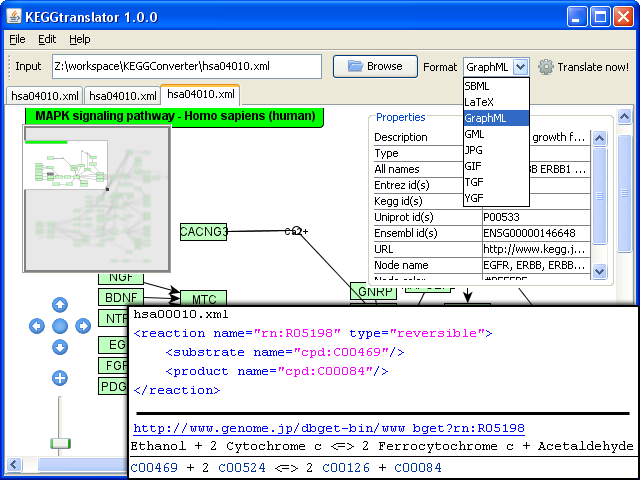
\includegraphics[width=1.0\columnwidth]{img/final.png}
%}
%\caption{Screenshot of KEGGtranslator. The list of all output formats is shown in the upper right corner. On the center, a translated GraphML pathway is displayed. The lower right corner demonstrates the need for autocompleting reactions: on the upper half, one can see the KGML-file with only one substrate and product. On the lower half, the complete reaction equation is shown. As one can see, one substrate and product is missing in the XML-document.}\label{fig:01}
%\end{figure}

%
%\begin{figure}[htb]%figure2
%\centerline{
%  \noindent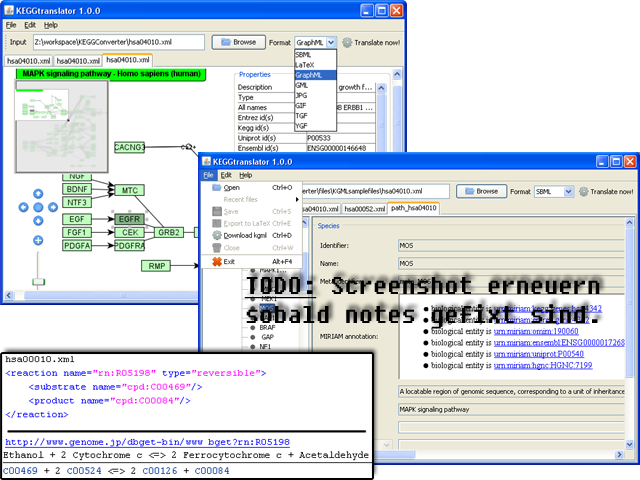
\includegraphics[width=1.0\columnwidth]{img/final2.png}
%}
%\caption{Alternative picture for Fig. \ref{fig:01}. We have to choose one of those.}\label{fig:02}
%\end{figure}

\section{Discussion}
%\section{Conclusion}
%(e.g., KEGGconverter \citep{KEGGconverter} and KEGG2SBML \citep{KEGG2SBML})
%(KEGGgraph \citep{KEGGgraph})
KEGGtranslator is a stand-alone application with a graphical user interface that runs on every operating system for which a Java\TTra virtual machine is available. There are other tools for converting KGML to SBML and for converting KGML to graph structures in R. But, to our knowledge, no other KEGG converter is able to translate KGML formatted files to such a variety of output formats with important functionalities like the autocompletion of reactions or the annotation of each element in the translated file, using various identifiers. Furthermore, KEGGtranslator is simple, easy-to-use and comes with a powerful command-line and graphical user interface.
The variety of output formats, combined with the translation options and comprehensive, standard-conform annotation of the pathway elements allow a quick and easy usage of files from the KEGG pathway database in a wide range of other applications.

%To our knowledge, these major deficiencies are not being corrected by other KEGG converters.
%In contrast to all other KEGG converting tools, KEGGtranslator comes with important functionalities like the autocompletion of reactions or the annotation of each element of the translated file, using various identifiers, and possesses a graphical user interface.

%Because of the variety of output formats, the pathways converted with KEGGtranslator can easily be opened in other applications. Further processing steps can be done quickly because a node or edge has much more information and identifier that just a name. And dynamic simulations on pathways can be done accurate with complete reactions.


%Because of these functionalities, the pathways converted with KEGGtranslator can easily be used for further processing. I.e. assigning

% Easy-to-use, help & tooptips, stand alone, java (systemunabhaengig)
%The application is purely written in java and makes use of the JSBML library. That makes it, in contrast to libSBML based applications, runnable on all operating systems that have a java virtual machine.


%TODO: Outlook: Webservice, libSBGN, (API)

\begin{figure}[h]%figure1
\centerline{
  \noindent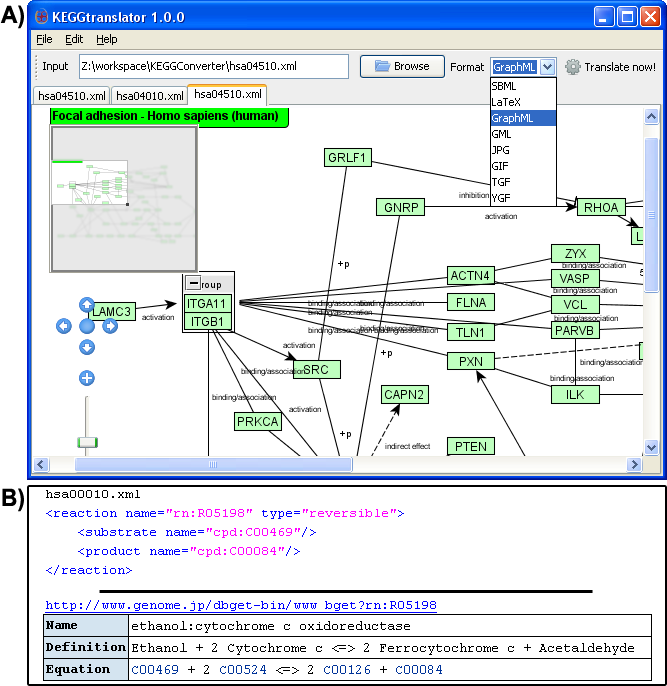
\includegraphics[width=0.95\columnwidth]{final3.png}
}
\caption{
%A) Screenshot of KEGGtranslator. The list of all output formats is shown in the upper right corner. On the center, a translated GraphML pathway is displayed. B) The need for autocompleting reactions: on the upper half, one can see the KGML-file with only one substrate and product. On the lower half, the complete reaction equation is shown. As one can see, one substrate and product is missing in the XML-document.
%The list of all output formats is shown in the upper right corner.
A) Screenshot of a translated GraphML pathway in KEGGtranslator. B) The need for autocompleting reactions: the upper half shows the KGML-file with only one substrate and product. On the lower half, the complete reaction equation is shown. As one can see, one substrate and product is missing in the XML-document.
}\label{fig:01}
\end{figure}

\section*{Acknowledgement}
We gratefully acknowledge very fruitful discussions with Jochen Supper, Akira Funahashi, and Toshiaki Katayama.\\
\emph{Funding\textcolon}
The Federal Ministry of Education and Research (BMBF, Germany) funded this work in the projects Spher4Sys (grant number 0315384C) and NGFNplus (grant number 01GS08134).

%\paragraph{Funding\textcolon} %Spher4Sys, BMBF, MARCAR, Virtualliver, NGFN
%\paragraph{Conflict of Interest\textcolon} none declared.

\bibliographystyle{natbib}
%\bibliographystyle{achemnat}
%\bibliographystyle{plainnat}
%\bibliographystyle{abbrv}
%\bibliographystyle{bioinformatics}
%\bibliographystyle{plain}
%\bibliography{Document}


%XXX: Uncomment for dynamic reference addition
%\bibliography{KEGGtranslator}


\begin{thebibliography}{}

\bibitem[Dr\"ager {\em et~al.}(2008)Dr\"ager, Hassis, Supper, Schr\"oder, and
  Zell]{SBMLSqueezer}
Dr\"ager, A. \emph{et al.} (2008).
\newblock {SBMLsqueezer: a CellDesigner plug-in to generate kinetic rate
  equations for biochemical networks}.
\newblock {\em BMC Systems Biology\/}, {\bf 2}(1), 39.

\bibitem[Dr\"ager {\em et~al.}(2009)Dr\"ager, Planatscher, Wouamba, Schr\"oder,
  Hucka, Endler, Golebiewski, M{\"u}ller, and Zell]{SBML2LaTeX}
Dr\"ager, A. \emph{et al.} (2009).
\newblock {SBML2\LaTeX: Conversion of SBML files into human-readable reports}.
\newblock {\em Bioinformatics\/}, {\bf 25}(11), 1455--1456.

\bibitem[Dr\"ager {\em et~al.}(2011)Dr\"ager, Rodriguez, D\"orr, Dumousseau,
  Wrzodek, Le~Nov\`{e}re, Zell, and Hucka]{JSBML}
Dr\"ager, A., Rodriguez, N. \emph{et al.} (2011).
\newblock {JSBML: a flexible and entirely Java-based library for working with
  SBML}.
\newblock {\em Submitted to Bioinformatics\/}.

\bibitem[Funahashi {\em et~al.}(2004)Funahashi, Jouraku, and Kitano]{KEGG2SBML}
Funahashi, A. \emph{et al.} (2004).
\newblock {Converting KEGG pathway database to SBML}.
\newblock {\em 8th Annual International Conference on Research in Computational
  Molecular Biology\/}.

\bibitem[Kanehisa and Goto(2000)Kanehisa and Goto]{Kanehisa2000}
Kanehisa, M. and Goto, S. (2000).
\newblock {KEGG: Kyoto Encyclopedia of Genes and Genomes}.
\newblock {\em Nucleic Acids Res\/}, {\bf 28}(1), 27--30.

\bibitem[{KEGG team}(2007){KEGG team}]{KEGGapi}
{KEGG team} (2007).
\newblock {\em KEGG API [{http://www.genome.jp/kegg/soap/}]\/}.

\bibitem[{KEGG team}(2010){KEGG team}]{KGML}
{KEGG team} (2010).
\newblock {\em {KEGG Markup Language [http://www.genome.jp/kegg/xml/docs]}\/}.

\bibitem[Moutselos {\em et~al.}(2009)Moutselos, Kanaris, Chatziioannou,
  Maglogiannis, and Kolisis]{KEGGconverter}
Moutselos, K. \emph{et al.} (2009).
\newblock {KEGGconverter: a tool for the in-silico modelling of metabolic
  networks of the KEGG Pathways database}.
\newblock {\em BMC Bioinformatics\/}, {\bf 10}, 324.

\bibitem[Nov\`{e}re {\em et~al.}(2005)Nov\`{e}re, Finney, Hucka, Bhalla,
  Campagne, Collado-Vides, Crampin, Halstead, Klipp, Mendes, Nielsen, Sauro,
  Shapiro, Snoep, Spence, and Wanner]{Novere2005}
Nov\`{e}re, N.~L. \emph{et al.} (2005).
\newblock Minimum information requested in the annotation of biochemical models
  {(MIRIAM)}.
\newblock {\em Nat Biotechnol\/}, {\bf 23}(12), 1509--1515.

\bibitem[Wiese {\em et~al.}(2001)Wiese, Eiglsperger, and Kaufmann]{yFiles}
Wiese, R. \emph{et al.} (2001).
\newblock {yFiles: Visualization and Automatic Layout of Graphs}.
\newblock {\em Proceedings of the 9th International Symposium on Graph Drawing
  (GD 2001)\/}%, pages 453--�454.

\bibitem[Zhang and Wiemann(2009)Zhang and Wiemann]{KEGGgraph}
Zhang, J.~D. and Wiemann, S. (2009).
\newblock {KEGGgraph: a graph approach to KEGG PATHWAY in R and bioconductor}.
\newblock {\em Bioinformatics\/}, {\bf 25}(11), 1470--1471.

\end{thebibliography}


\end{document}
